\documentclass[]{standalone}

\usepackage{amsmath}
\usepackage{amsfonts}
\usepackage{amssymb}
\usepackage{graphicx}
\usepackage{tikz}
\usepackage{import}
\usepackage[subpreambles=true]{standalone}

\usepackage{tikz}
\usepackage{tikz-3dplot}

\usetikzlibrary{positioning}

\begin{document}

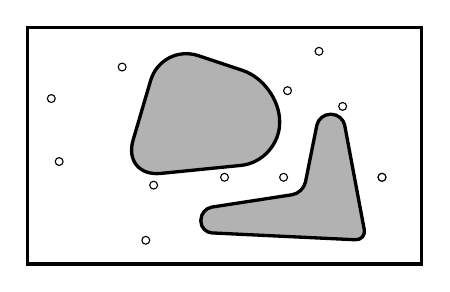
\begin{tikzpicture}[scale=1]
    % \path[draw, fill] (5.5, 3.0) circle (0.05) node[right]{$V_\mathrm{closed}$};
    % \path[draw, fill=gray] (5.5, 2.5) circle (0.05) node[right]{$V_\mathrm{open}$};
    % \path[draw, fill=white] (5.5, 2.0) circle (0.05) node[right]{$V_\mathrm{unvisited}$};

    \useasboundingbox (0,0) rectangle (5,3);

    \coordinate (init) at (0.5,0.5);
    \coordinate (goal) at (4.6,2.25);
    \coordinate (obs1) at (2.4,2.1);
    \coordinate (obs2) at (3.7,0.65);
    \coordinate (n0) at (0.4,1.3);
    \coordinate (n1) at (1.2,2.5);
    \coordinate (n2) at (1.5,0.3);
    \coordinate (n3) at (4.5,1.1);
    \coordinate (n4) at (1.6,1.0);
    \coordinate (n5) at (4.0,2.0);
    \coordinate (n6) at (3.3,2.2);
    \coordinate (n7) at (3.25,1.1);
    \coordinate (n8) at (2.5,1.1);
    \coordinate (n9) at (0.3,2.1);
    \coordinate (n10) at (3.7,2.7);

    \path[draw, fill=white] (n0) circle (0.05);
    \path[draw, fill=white] (n1) circle (0.05);
    \path[draw, fill=white] (n2) circle (0.05);
    \path[draw, fill=white] (n3) circle (0.05);
    \path[draw, fill=white] (n4) circle (0.05);
    \path[draw, fill=white] (n5) circle (0.05);
    \path[draw, fill=white] (n6) circle (0.05);
    \path[draw, fill=white] (n7) circle (0.05);
    \path[draw, fill=white] (n8) circle (0.05);
    \path[draw, fill=white] (n9) circle (0.05);
    \path[draw, fill=white] (n10) circle (0.05);

    % \visible<1>{
    % \begin{scope}
    %     \clip (0,0) rectangle (5,3);
    %     \path[draw, thick, dashed, fill=gray, fill opacity=0.2] (init) circle (1.3);
    % \end{scope}}

    % \visible<2-3>{
    % \begin{scope}
    %     \clip (0,0) rectangle (5,3);
    %     \path[draw, thick, dashed, fill=gray, fill opacity=0.2] (n0) circle (1.3);
    % \end{scope}}

    % \visible<4-5>{
    % \begin{scope}
    %     \clip (0,0) rectangle (5,3);
    %     \path[draw, thick, dashed, fill=gray, fill opacity=0.2] (n4) circle (1.3);
    % \end{scope}}

    % \visible<6-7>{
    % \begin{scope}
    %     \clip (0,0) rectangle (5,3);
    %     \path[draw, thick, dashed, fill=gray, fill opacity=0.2] (n2) circle (1.3);
    % \end{scope}}

    % \visible<9>{
    % \begin{scope}
    %     \clip (0,0) rectangle (5,3);
    %     \path[draw, thick, dashed, fill=gray, fill opacity=0.2] (n0) circle (1.3);
    % \end{scope}}

    % \visible<10-11>{
    % \begin{scope}
    %     \clip (0,0) rectangle (5,3);
    %     \path[draw, thick, dashed, fill=gray, fill opacity=0.2] (n9) circle (1.3);
    % \end{scope}}

    % \visible<3->{
    % \path[draw] (n0) -- (init);}
    % \visible<5->{
    % \path[draw] (n4) -- (init);}
    % \visible<7->{
    % \path[draw] (n2) -- (init);}
    % \visible<11->{
    % \path[draw] (n0) -- (n9);}
    % \visible<13->{
    % \path[draw] (n9) -- (n1);
    % \path[draw] (n4) -- (n8);
    % \path[draw] (n8) -- (n7);
    % \path[draw] (n7) -- (n6);
    % \path[draw] (n6) -- (n10);
    % \path[draw] (n6) -- (n5);
    % \path[draw] (n6) -- (goal);}

    % \visible<14->{
    % \path[draw=red, thick] (init) -- (n4) -- (n8) -- (n7) -- (n6) -- (goal);}

    % \visible<1-7>{\path[draw, fill=gray] (init) circle (0.05) node[below] {$x_\mathrm{init}$};}
    % \visible<8->{\path[draw, fill=black] (init) circle (0.05) node[below] {$x_\mathrm{init}$};}

    % \visible<1-12>{\path[draw, fill=white] (goal) circle (0.05) node[above] {$x_\mathrm{goal}$};}
    % \visible<13->{\path[draw, fill=gray] (goal) circle (0.05) node[above] {$x_\mathrm{goal}$};}

    % \visible<1-7>{\path[draw, fill=white] (n0) circle (0.05);};
    % \visible<8-11>{\path[draw, fill=gray] (n0) circle (0.05);};
    % \visible<12->{\path[draw, fill=black] (n0) circle (0.05);};


    % \visible<1-12>{\path[draw, fill=white] (n1) circle (0.05);};
    % \visible<13->{\path[draw, fill=black] (n1) circle (0.05);};

    % \visible<1-7>{\path[draw, fill=white] (n2) circle (0.05);};
    % \visible<8->{\path[draw, fill=gray] (n2) circle (0.05);};
    % \visible<13->{\path[draw, fill=black] (n2) circle (0.05);};

    \path[draw, fill=white] (n3) circle (0.05);

    % \visible<1-7>{\path[draw, fill=white] (n4) circle (0.05);};
    % \visible<8->{\path[draw, fill=gray] (n4) circle (0.05);};
    % \visible<13->{\path[draw, fill=black] (n4) circle (0.05);};

    % \visible<1-12>{\path[draw, fill=white] (n5) circle (0.05);}
    % \visible<13->{\path[draw, fill=gray] (n5) circle (0.05);}

    % \visible<1-12>{\path[draw, fill=white] (n6) circle (0.05);}
    % \visible<13->{\path[draw, fill=black] (n6) circle (0.05);}

    % \visible<1-12>{\path[draw, fill=white] (n7) circle (0.05);}
    % \visible<13->{\path[draw, fill=black] (n7) circle (0.05);}

    % \visible<1-12>{\path[draw, fill=white] (n8) circle (0.05);}
    % \visible<13->{\path[draw, fill=black] (n8) circle (0.05);}

    % \visible<1-11>{\path[draw, fill=white] (n9) circle (0.05);}
    % \visible<12->{\path[draw, fill=gray] (n9) circle (0.05);}
    % \visible<13->{\path[draw, fill=black] (n9) circle (0.05);}

    % \visible<1-12>{\path[draw, fill=white] (n10) circle (0.05);}
    % \visible<13->{\path[draw, fill=gray] (n10) circle (0.05);}


    \path[draw, very thick] (0,0) -- (5,0) -- (5,3) -- (0,3) -- cycle;


    \path[draw, very thick, rounded corners=14pt, fill=black!30] (obs1) ++(-1.2,-1) -- ++(2,0.2) -- ++(0,1) -- ++(-1.5,0.5) -- cycle;
    \path[draw, very thick, rounded corners=4pt, fill=black!30] (obs2) ++(-1.5,-0.25) -- ++(0,0.3) -- ++(1.3,0.2) -- ++(0.2,1) -- ++(0.3,0) -- ++(0.3,-1.6) -- cycle;

\end{tikzpicture}
\end{document}